\let\negmedspace\undefined
\let\negthickspace\undefined
\documentclass[journal,12pt,twocolumn]{IEEEtran}
\usepackage{cite}
\usepackage{amsmath,amssymb,amsfonts,amsthm}
\usepackage{algorithmic}
\usepackage{graphicx}
\usepackage{textcomp}
\usepackage{xcolor}
\usepackage{txfonts}
\usepackage{listings}
\usepackage{enumitem}
\usepackage{mathtools}
\usepackage{gensymb}
\usepackage{comment}
\usepackage[breaklinks=true]{hyperref}
\usepackage{tkz-euclide} 
\usepackage{listings}
\usepackage{gvv}                                        
\def\inputGnumericTable{}                                 
\usepackage[latin1]{inputenc}                                
\usepackage{color}                                            
\usepackage{array}                                            
\usepackage{longtable}                                       
\usepackage{calc}                                             
\usepackage{multirow}                                         
\usepackage{hhline}                                           
\usepackage{ifthen}                                           
\usepackage{lscape}

\newtheorem{theorem}{Theorem}[section]
\newtheorem{problem}{Problem}
\newtheorem{proposition}{Proposition}[section]
\newtheorem{lemma}{Lemma}[section]
\newtheorem{corollary}[theorem]{Corollary}
\newtheorem{example}{Example}[section]
\newtheorem{definition}[problem]{Definition}
\newcommand{\BEQA}{\begin{eqnarray}}
\newcommand{\EEQA}{\end{eqnarray}}
\newcommand{\define}{\stackrel{\triangle}{=}}
\theoremstyle{remark}
\newtheorem{rem}{Remark}


\title{Assignment-2 SequenceAndSeries}
\author{Deepak Reddy ee23btech11047}
\date{January 2024}

\begin{document}

\maketitle
\section*{Exercise 9.1}
\textbf{Question:}\\
Write the first five terms of each of the sequences in Exercises 1 to 6 whose $n^{th}$
terms are:\\
4. $x(n) = \frac{2n-3}{6}$\\
\textbf{Solution:}\\
$n^{th}$ term of the sequence is given by the above expression\\
we use n=0, we get
\begin{align} x(0) = \frac{2 \times 0 - 3}{6} = \frac{-1}{2} \end{align}\\
we use n=1, we get First Term,
\begin{align} x(1) = \frac{2 \times 1 - 3}{6} = \frac{-1}{6} \end{align}\\
Similarly we will find other terms like this\\
we use n=2, we get Second Term,
\begin{align} x(2) = \frac{2 \times 2 - 3}{6} = \frac{1}{6}  \end{align}\\
we use n=3, we get Third Term,
\begin{align} x(3) = \frac{2 \times 3 - 3}{6} = \frac{1}{2} \end{align}\\
we use n=4, we get Fourth Term,
\begin{align} x(4) = \frac{2 \times 4 - 3}{6} = \frac{5}{6} \end{align}\\
Therefore, The first five terms of the given sequence are
$x(0) = \frac{-1}{2}, x(1) = \frac{-1}{6},x(2) = \frac{1}{2}, x(3) = \frac{1}{2} , x(4) = \frac{5}{6}.$\\
\\
To express x(n) in terms of u(n) we can express it as 
\begin{align} x(n) = \frac{2n-3}{6} = \left(\frac{n}{3} - \frac{1}{2} \right)\cdot u(n) \end{align}
\bigskip
Now lets find Z transform of x(n)
\begin{align} X(Z) = \sum_{n = -\infty}^{\infty} x(n) \cdot Z^{-n} \end{align}
\bigskip
Now substitute the expression of 
$x(n) = \left(\frac{n}{3} - \frac{1}{2} \right)\cdot u(n)$ into the Z-Transform Formula:
\begin{align} X(Z) = \sum_{n = -\infty}^{\infty} (\frac{n}{3} - \frac{1}{2} ) \cdot u(n)  \cdot Z^{-n} \end{align}
\bigskip
Now we can write it as 
\begin{align} X(Z) = \sum_{n=0}^{\infty} \frac{n}{3} \cdot Z^{-n} - \sum_{n=0}^{\infty} \frac{1}{2} \cdot Z^{-n} \end{align}
\bigskip
Now we will find the both summations 
\begin{align} \sum_{n=0}^{\infty} \frac{n}{3} \cdot Z^{-n} = \frac{1}{3} \cdot (0 + 1.Z^{-1} + 2.Z^{-2} + \ldots) \end{align}
\bigskip
Now if we multiply the above equation by $Z^{-1}$ we get 
\begin{align} Z^{-1} \cdot \sum_{n=0}^{\infty} \frac{n}{3} \cdot Z^{-n} =\frac{1}{3} \cdot (1.Z^{-2} + 2.Z^{-3} + \ldots ) \end{align}
\bigskip
Now if we subtract the above two equations we get 
\begin{align} \sum_{n=0}^{\infty} \frac{n}{3} \cdot Z^{-n} = \frac{Z}{Z-1} \cdot \frac{1}{3} \cdot (Z^{-1} + Z^{-2} + Z^{-3} + \ldots) \end{align}
\begin{align} \sum_{n=0}^{\infty} \frac{n}{3} \cdot Z^{-n} = \frac{1}{3} \cdot \left(\frac{Z}{(Z-1)^{2}}\right) \end{align}

\begin{align} \sum_{n=0}^{\infty} \frac{1}{2} \cdot Z^{-n} = \frac{1}{2} \cdot (1+Z^{-1} + Z^{-2} + \ldots) = \frac{1}{2} \cdot \frac{1}{1- Z^{-1}} \end{align}
\newpage
So now Z transform of the x(n) is 
\begin{align} X(Z) = \frac{1}{3} \cdot \frac{Z}{(Z-1)^{2}} - \frac{1}{2} \cdot \frac{1}{1-Z^{-1}} \end{align}
\begin{align} X(Z) = {\frac{5Z-3 Z^{2}}{6(Z-1)^{2}}} \end{align}

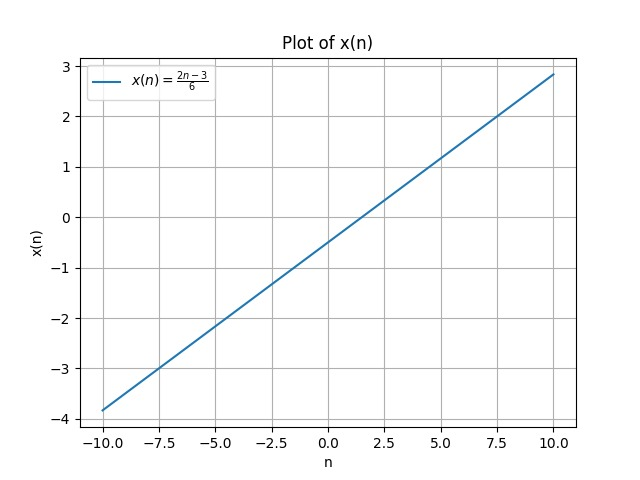
\includegraphics[width=0.55\textwidth]{figs/graphgvv1.jpg}
\end{document}
